\section{Data view}

\subsection{Mission}
Databasen har til formål at, hjælpe brugeren overskue hvilke droner han har til rådighed. Se hvilke status de har i systemet, om de er ude og flyve eller om de er i dock. Databasen trackker også hvilke events der forgår på nuværende tidspunkt og historik over events. Tilhørende events er information omkring flyve ruten, billeder tager på turen samt en log.

\subsection{Design}
På figuren \ref{fig:database_design} ses designet af databasen. Som beskrevet tidligere er database typen en SQLight database. Alt kommunikation til og fra databasen vil fungere igennem et database API som ligger på serveren. Hvert tabel vil blive beskrevet mere detaljeret under dette afsnit.

\vspace{-5pt}
\begin{figure}[H]
	\centering
	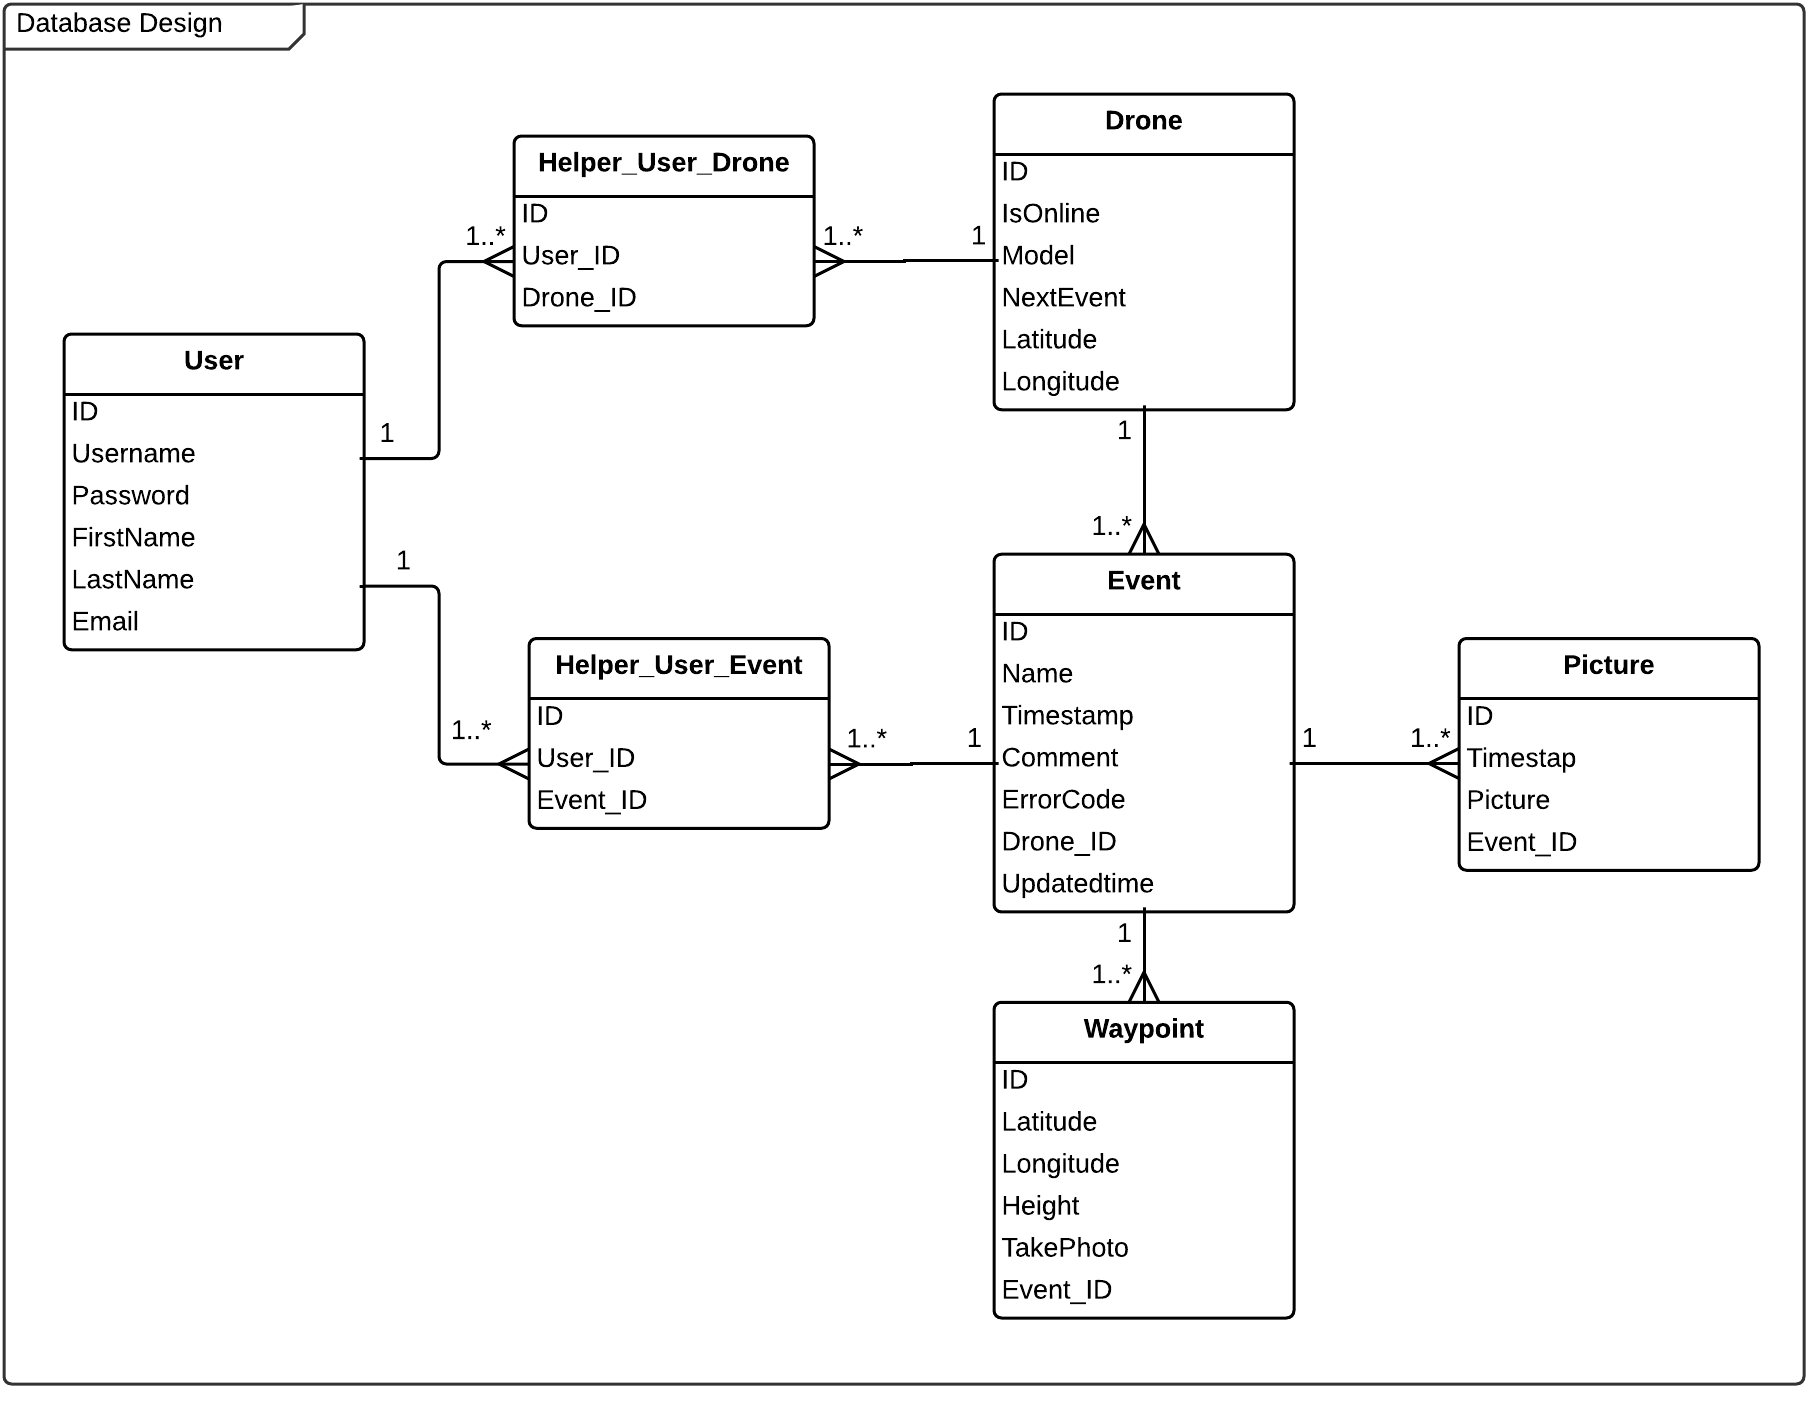
\includegraphics[width=1\textwidth]{Billeder/database/database_design.png}
	\vspace{-5pt}
	\caption{Database design}
	\label{fig:database_design}
\end{figure}

\newpage
\subsection{Database detaljeret beskrivelse}

\subsubsection{User tabel}
Tabellen indeholder data om den givet bruger i systemet. Tabellen giver også mulighed for brugeren at tilgå dronerne, events og de gemte ruter i systemet, via tabellens Foring keys.
\vspace{-5pt}
\begin{figure}[H]
	\centering
	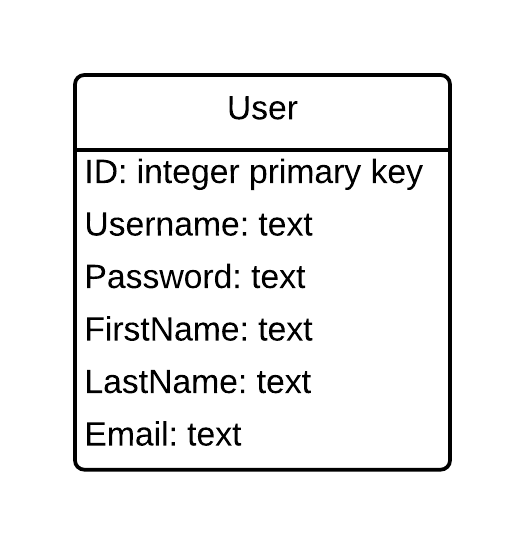
\includegraphics[width=0.5\textwidth]{Billeder/database/UserTabel.png}
	\vspace{-5pt}
	\caption{User tabel}
	\label{fig:user_tabel}
\end{figure}

\begin{table}[H]
\begin{tabular}{| p{3cm}| p{11.5cm}|}
\hline

Formål	 							& Holde data om brugeren i systemet, samt tjekke om brugeren eksterre ved forsøg på login.\\\hline
Forbindelser						& Tabellen har tre Foring keys til Helper\_User\_Drone og Helper\_User\_Event hjælpe tabellerne.\\\hline
Attributter						& \begin{itemize}
												\item ID: Primary key.
												\item Username: Brugernavnet til systemet.
												\item Password: Brugerens kode.
												\item FirstName: Brugers fornavn.
												\item LastName: Brugerens efternavn.
												\item Email: Brugerens email adresse.
											\end{itemize} \\\hline 
\end{tabular}
\caption{Fejlmode \#1 - Ingen GPS signal}
\label{tab:fejlmode1}
\end{table}

